% File: cambiamenti.tex
% Created: 2015-01-22
% Author: Tesser Paolo
% Email: p.tesser921@gmail.com
% 
%
% Modification History
% Version	Modifier Date	Author			Change
% ====================================================================
% 0.0.1		2015-01-22		Tesser Paolo	inserita sezione capitolo
% ====================================================================
% 0.0.2		2015-01-28		Tesser Paolo	spiegazione pack objrem + diagramma
% ====================================================================
% 0.0.3		2015-01-29		Tesser Paolo	spiegazione metodi e membri ObjRemImpl
% ====================================================================
%


\section{Cambiamenti e Aggiunte} % (fold)
\label{sec:cambiamenti_e_aggiunte}
In questa sezione verranno descritti i cambiamenti e le aggiunte apportate alla precedente versione per permettere al programma di essere distribuito tra un server e più client (come evidenziato nella sezione \ref{sec:note_introduttive}). \\
Non sono state effettuate particolare revisioni al codice sviluppato per soddisfare i requisiti della seconda parte. \\
\'E stata cancellata solo la classe \textbf{PuzzleSolver}, responsabile dell'esecuzione del programma, non più necessaria, a favore di due nuove classi: \textbf{PuzzleSolverServer} e \textbf{PuzzleSolverClient}, responsabili dell'esecuzione del programma sul server e di quello sul client. Nella sezione \ref{sec:logica_di_comunicazione_client_server} verrà illustrato quale compito svolgono attraverso il loro main queste classi.

	\subsection{Aggiunte} % (fold)
	\label{sub:aggiunte}
		\subsubsection{Package objrem} % (fold)
		\label{ssub:package_objrem}
		Questo package contiene le classi che servono per permettere al client che lo desidera, di lavorare con il server per la risoluzione di un puzzle. \\
		\'E presente un'interfaccia condivisa sia dal server che dal client: \textbf{ObjRem}, la quale estende la classe Remote del package rmi. Questa è l'unica cosa che sarà disponibile al client per lanciare i metodi che consentiranno la codifica del puzzle nel server. \\
		Nel server verrà implementata l'interfaccia precedente dalla classe \textbf{ObjRemImpl}, che darà una definizione concreta dei metodi e aggiungerà dei membri. Di seguito viene spiegata la loro funzione. \\ \\
		\textbf{Membri}:
			\begin{itemize}
				\item \textbf{NUMCLIENT}: membro statico intero che serve a tenere il conto di quanti client hanno fatto richiesta al server di un identificativo. Questo garantisce che ogni richiesta sia associata ad un valore diverso e non ci sia conflitto tra client diversi;
				\item \textbf{clients}: membro di tipo HashMap<String, Puzzle>. Serve per immagazzinare il puzzle che ciascun client vuole risolvere, associandolo all'identificativo che viene associato al client al momento dell'avvio del programma;
				\item \textbf{output}: membro di tipo HashMap<String, ArrayList<String> >. Serve per immagazzinare il puzzle risolto nel formato richiesto dal client, cioè ArrayList<String>, per scriverlo poi sul file di output;
				\item \textbf{solveThread}: membro di tipo HashMap<String, SolveThread>. Serve per immagazzinare la lista dei thread avviati per la risoluzione dei diversi puzzle. Questo ci consente in seguito di usarlo per fare delle chiamate del metodo \textbf{join()} sul thread lanciato, per mettere in attesa un altro thread fintanto che l'operazione non è completata;
				\item \textbf{concreteThread}: membro di tipo HashMap<String, ConcreteThread>. Serve per immagazzinare la lista dei thread avviati per la conversione dei diversi puzzle. Questo ci consente in seguito di usarlo per fare delle chiamate del metodo \textbf{join()} sul thread lanciato, per mettere in attesa un altro thread fintanto che l'operazione non è completata.
			\end{itemize}
		\noindent \\
		\textbf{Metodi}:
			\begin{itemize}
				\item \textbf{getNewIdClient()}: ritorna un identificativo univoco di tipo stringa, formato dalla parola client più il numero del prossimo client disponibile tramite l'accesso al membro \textbf{NUMCLIENT};
				\item \textbf{setClientPuzzle(String, ArrayList<String>)}: riceve un ArrayList dal client, rappresentativa del puzzle che vuole risolvere. A partire da essa crea un nuovo puzzle e lo mappa nel membro \textbf{clients}, dandogli come chiave l'identificativo del client ricevuto in input e come valore quello del puzzle appena creato;
				\item \textbf{solve(String, String)}: imposta la tipologia di ordinamento del puzzle in base al valore ricevuto dal client. Crea e lancia un thread di tipo SolveThread che andrà a risolvere il puzzle del client che lo ha richiesto. Inoltre, prima di eseguire il thread, lo aggiunge nel membro \textbf{solveThread};
				\item \textbf{convert(String)}: crea un thread del tipo ConvertThread e lo aggiunge al membro \textbf{concreteThread}, ma lo avvia solo dopo che il thread lanciato per la risoluzione del puzzle ha terminato la sua esecuzione;
				\item \textbf{getOutput(String)}: restituisce un ArrayList di stringhe che servono al client per scrivere su file il puzzle nella forma richiesta dalla specifica;
				\item \textbf{getPuzzleCol(String)}: restituisce il numero di colonne presenti nel puzzle che il client ha richiesto di risolvere;
				\item \textbf{getPuzzleRow(String)}: restituisce il numero di righe presenti nel puzzle che il client ha richiesto di risolvere.
			\end{itemize}
		\noindent
		\textbf{Nota}: tutti i metodi elencati sono \textbf{synchronized} per garantire che non ci sia interferenza tra i diversi client possibili. \\
		Il primo parametro formale dei metodi elencati (qualora ci fosse) è sempre la stringa identificativa del client, ricevuta all'inizio dalla chiamata del metodo \textbf{getNewIdClient()}.
		
		\begin{figure}[htbp]
			\centering
			\centerline{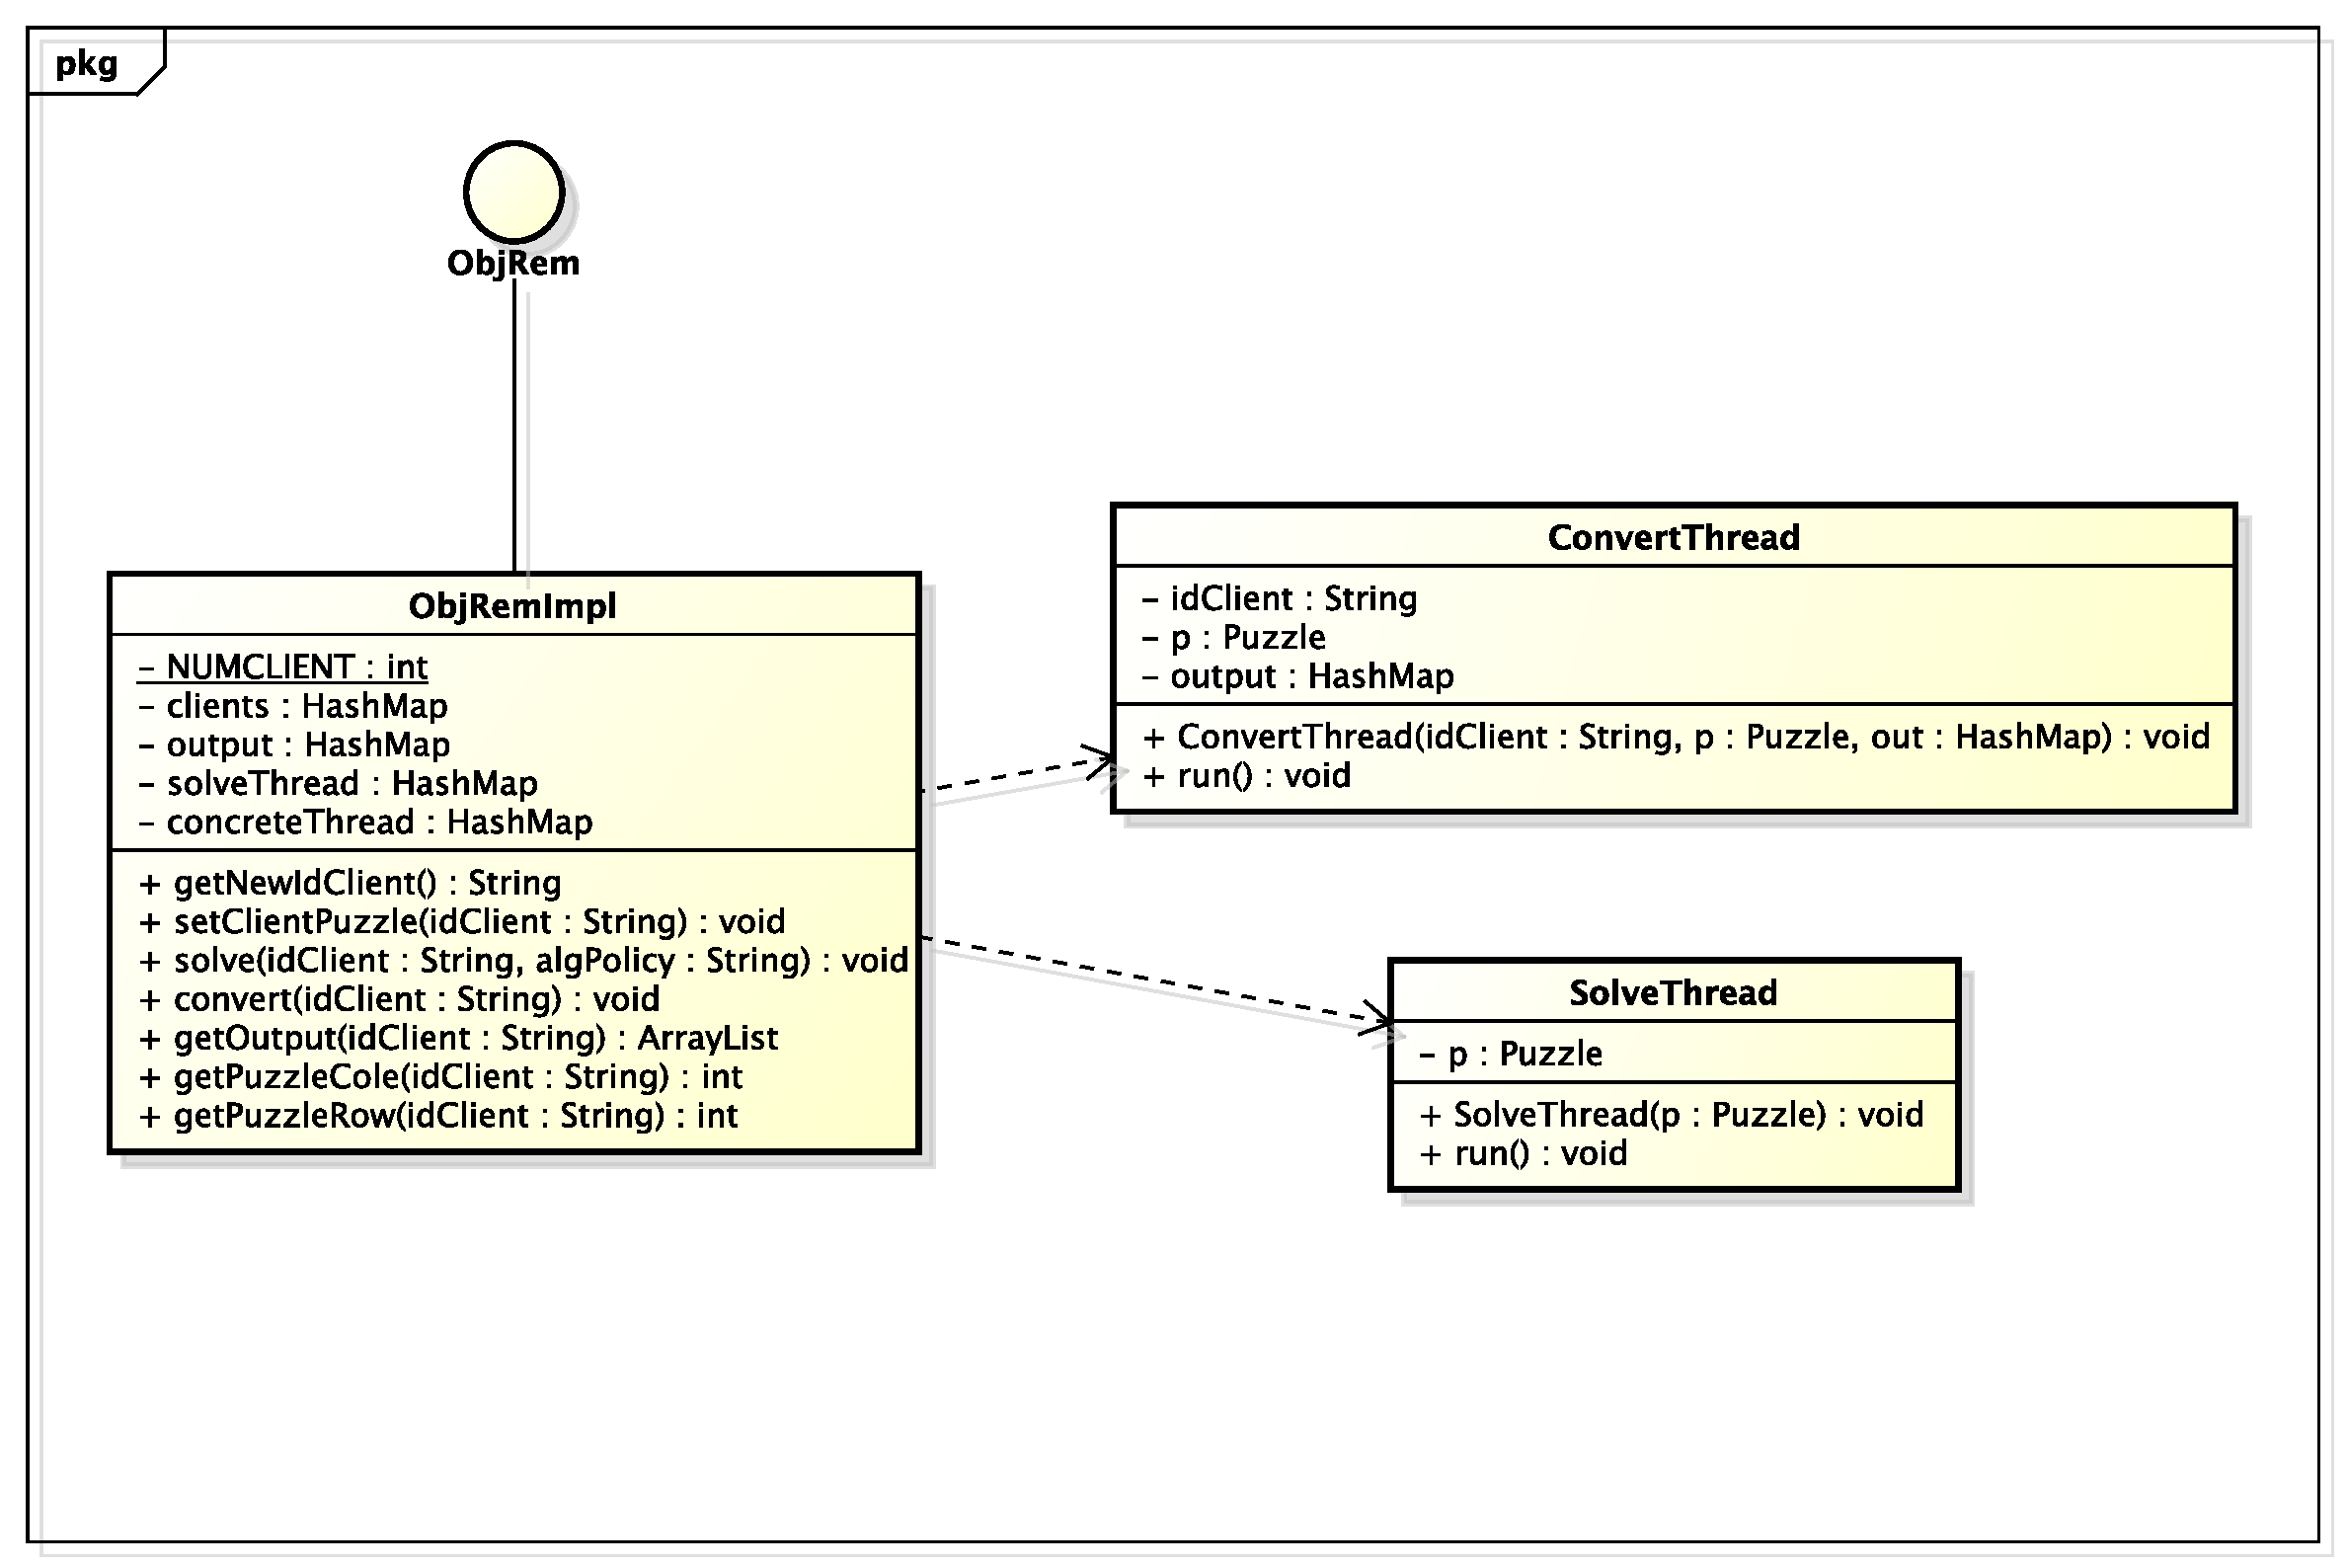
\includegraphics[scale=0.5]{img/objrem.pdf}}
			\caption{Diagramma delle classi - Package objrem}
			\label{fig_package_objrem}
		\end{figure}
		
		% subsubsection package_objrem (end)
	% subsection aggiunte (end)
% section cambiamenti_e_aggiunte (end)



